% \section{Method}
% \label{headings}

% The most straightforward way to let LLMs interact with Knowledge Graphs is through retrieval augmented generation (RAG), where a retriever fetches related information from graphs as context for LLM generation. Source documents are pre-processed and indexed using an embedding model. At inference time, the query is embedded using the same embedding model and the resulting vector is compared to all the previously indexed vectors. The resulting context is passed to the LLM for generation. A key issue with this approach is that relevant information is often spread across documents meaning that the LLM could miss crucial information. Motivated by this distributed information problem, GraphRAG utilizes a knowledge graph as the backbone of the retrieval process. External knowledge is embedded into a knowledge graph and either the content of a single node in the graph, or a local subgraph can be passed as context to the LLM. 

% Information in knowledge graphs lies in the interconnections between vertices which necessitates traversing the knowledge graph. To this end, previous work shows that LLMs can achieve good performance by enabling LLM's to interact with a knowledge graph iteratively. We extend this iterative approach due to its effectiveness and compatibility with our inference scaling strategies. Next, we discuss each step in the graph traversal process. 

% {\bf Reasoning. } Given a question or previous interactions, the LLM first proposes a thought about what information is still needed to answer the question or if the question can be answered with the current context. For example, for the question “Who are the authors of Language Models are Unsupervised Multitask Learners?”. The LLMs are expected to reason “We need to first find the paper node {Language Models are Unsupervised Multitask Learners} on the graph.” 

% {\bf Interaction. } Based on the output of all the previous reasoning and interaction steps, the LLM generates an interaction with the knowledge graph. We follow the structure of Graph-CoT and pre-define four functions that allow the LLM to retrieve information. 
% \begin{itemize}
%     \item {\it RetrieveNode}: Retrieves the most similar node using semantic search (This is identical to performing standard RAG on the knowledge graph)
%     \item {\it NodeFeature}: extract the feature information for a given node. 
%     \item {\it NeighborCheck}: returns information about the neighbors of a given node. 
%     \item {\it NodeDegree}: returns the degree of a given node. 
% \end{itemize}
% The LLM is tasked with generating correct function calls for the knowledge graph. {\bf say something about the connection to agents idk what to say rn though}
% \subsection{Inference scaling}
% The structure of knowledge graphs necessitates multi-hop reasoning to be able to effectively perform question answering. This is because information is held within the connections of the graph and not necessarily within individual nodes. Answering a question could require multiple hops from a source node in order to gather all necessary information. Solving this problem is exacerbated due to {\it graph size explosion} where the size of the local subgraph increases exponentially as the number of hops from the source node increases. LLMs traditionally struggle with these types of hard reasoning problems. Figure 2 shows that as the number of hops from the source node increases performance is drastically reduced   

% \begin{figure}
%   \centering
%   \includegraphics[width=0.6\textwidth]{img/multi_hop_reasoning.png}
%   \caption{\textcolor{blue}{This is the figure from Graph-CoT paper need to replace with my own}, just here for now. Performance of Graph-CoT on different difficulty levels in GRBench Dataset. Easy Questions refer to those that can be answered with a single hop. Medium are those that can be answered with multi-hop reasoning. Hard call for inductive reasoning with information from the graph as context}
% \end{figure}

% To solve this challenge, we propose scaling up inference compute thereby improving the reasoning ability of our LLM. Recent works have shown that scaling up the inference time compute of LLMs can dramatically improve performance on a variety of hard reasoning problems such as advanced math or coding. Two classes of inference scaling exist, {\bf sequential scaling} and {\bf parallel scaling}. We experiment with applying both sequential scaling and parallel scaling to the graph-reasoning domain. 

% {\bf 1.) Sequential scaling} conditions the current computation on previous ones. This is typically achieved through a long chain-of-thought or reasoning trace. This long chain-of-thought allows the model to build on intermediate results, and iteratively refine its answer. We utilize sequential scaling by scaling the number of interactions our LLM is able to make with the knowledge graph. This explicitly increases the length of the models chain of thought and allows it to more freely explore the graph. 

% {\bf 2.) Parallel scaling} involves sampling multiple responses from the model and utilizing a pre-defined selection criterion for picking the best response. The most straightforward approach is majority voting, or self consistency, where multiple responses are sampled from the model and the most common responses is picked. Other methods like best-of-N rely on a separate verifier to rank responses and then select the best one. We opt to utilize majority voting due to its lack of reliance on external verification. Specifically, we perform majority voting on the generated {\bf interaction} with the knowledge graph. . 

% {\textcolor{blue}{ SAY SOMETHING HERE ABOUT BUDGET FORCING}} Since we control how many steps our model is able to take on the graph, our method is consistent with recent work on budget forcing. That is, we are able to precisely control how much compute our model is able to use at inference time.   



\section{Method}
\label{sec:method}

Retrieval-augmented generation (RAG) \citep{gao2024retrievalaugmentedgenerationlargelanguage, lewis2020retrieval} is a widely used method to integrate large language models (LLMs) with external knowledge sources. In this framework, source documents are embedded and indexed during preprocessing. At inference time, a query is embedded using the same model, and its nearest neighbors are retrieved to form a contextual prompt for the LLM. However, a key limitation of traditional RAG is that relevant information is often distributed across multiple documents. This fragmentation can hinder the LLM’s ability to synthesize a complete and accurate response.

To address this issue, we build on GraphRAG, which leverages a knowledge graph (KG) as the backbone of the retrieval process. In this setting, external knowledge is structured as a graph, and subgraphs, rather than isolated documents, are used as context for the LLM. This representation captures relational structure and enables richer contextualization. Information in KGs often resides in the relationships between nodes, necessitating multi-hop reasoning and graph traversal to answer complex queries. Prior work has shown that LLMs can effectively engage with KGs through iterative reasoning and interaction \citep{jin2024graph}. We extend this paradigm and enhance it with inference-time scaling strategies to improve performance on reasoning-intensive tasks.

\subsection{Graph traversal with LLMs}

Our framework, shown in figure \ref{fig:ISGR_overview}, follows an iterative reasoning and interaction loop between the LLM and the KG, enabling compositional and multi-hop reasoning. Each iteration consists of two phases:


% \begin{figure}[t]
% \centering
%     \begin{subfigure}[t]{0.48\textwidth}
%         \centering
%         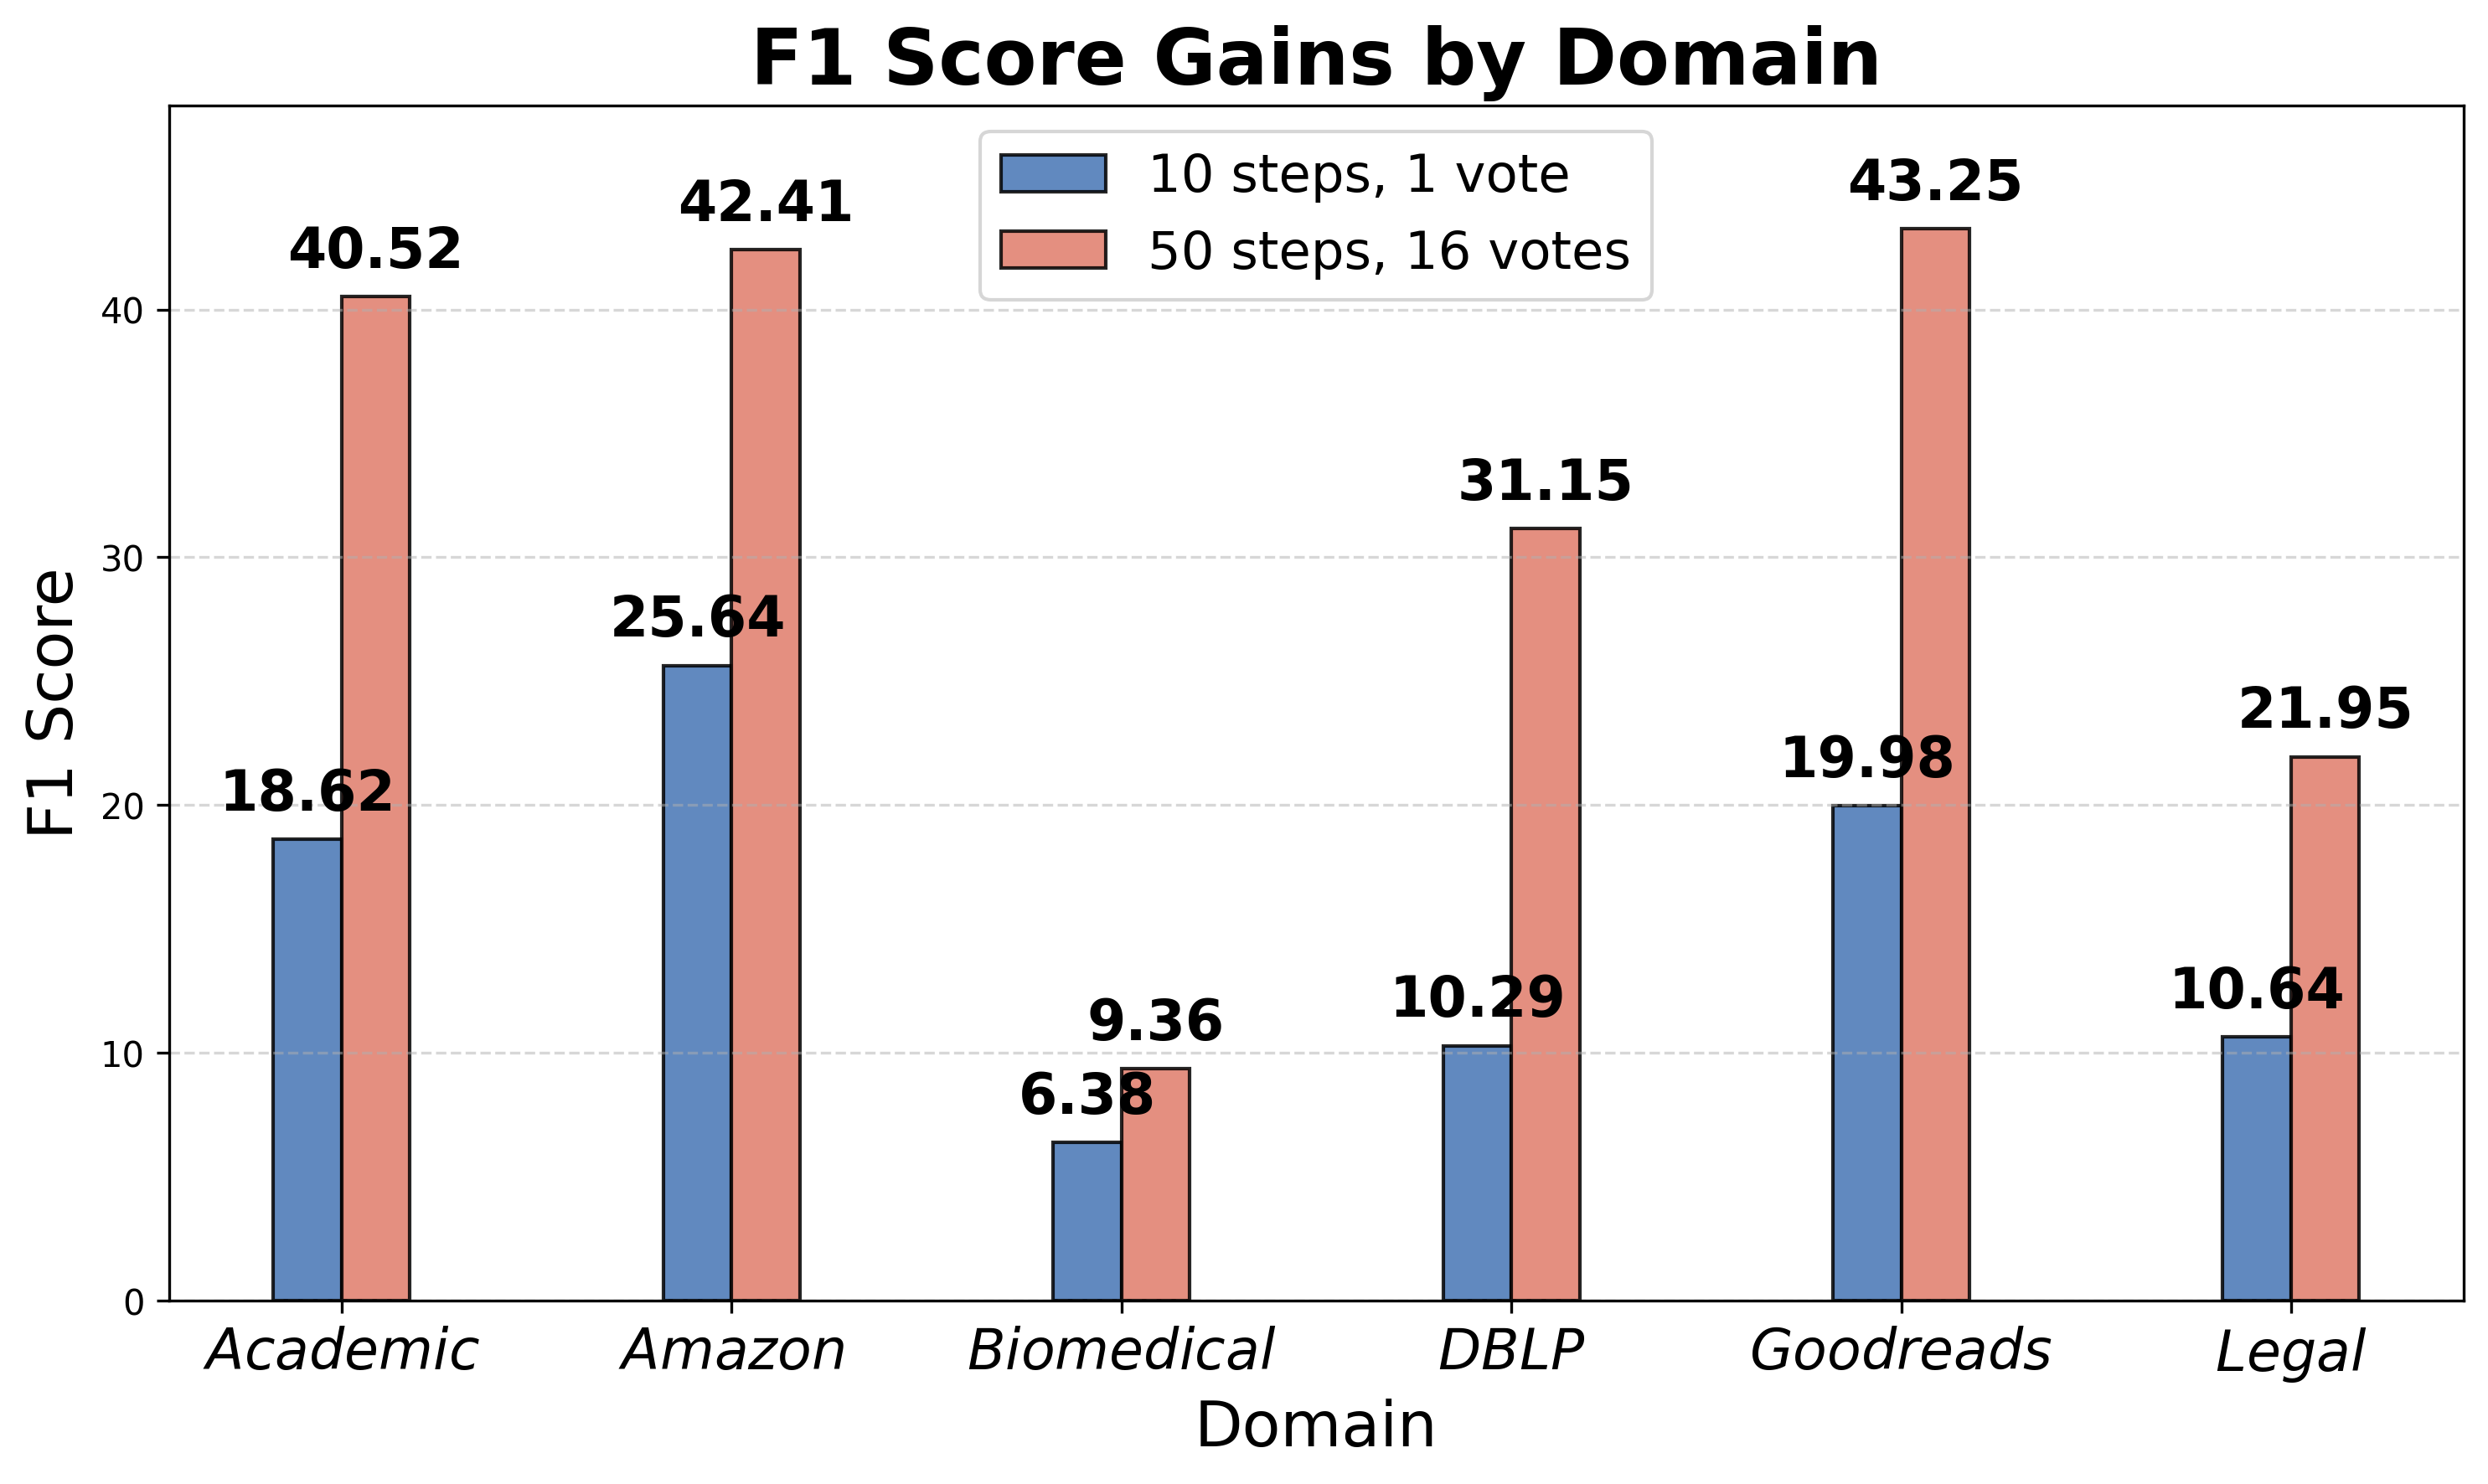
\includegraphics[width=\textwidth]{img/f1_score_medium_hard_avg_domain_bar_chart.png}
%         \caption{F1 scores on medium and hard questions}
%         \label{fig:multi-hopf1}
%     \end{subfigure}
%     \begin{subfigure}[t]{0.48\textwidth}
%         \centering
%         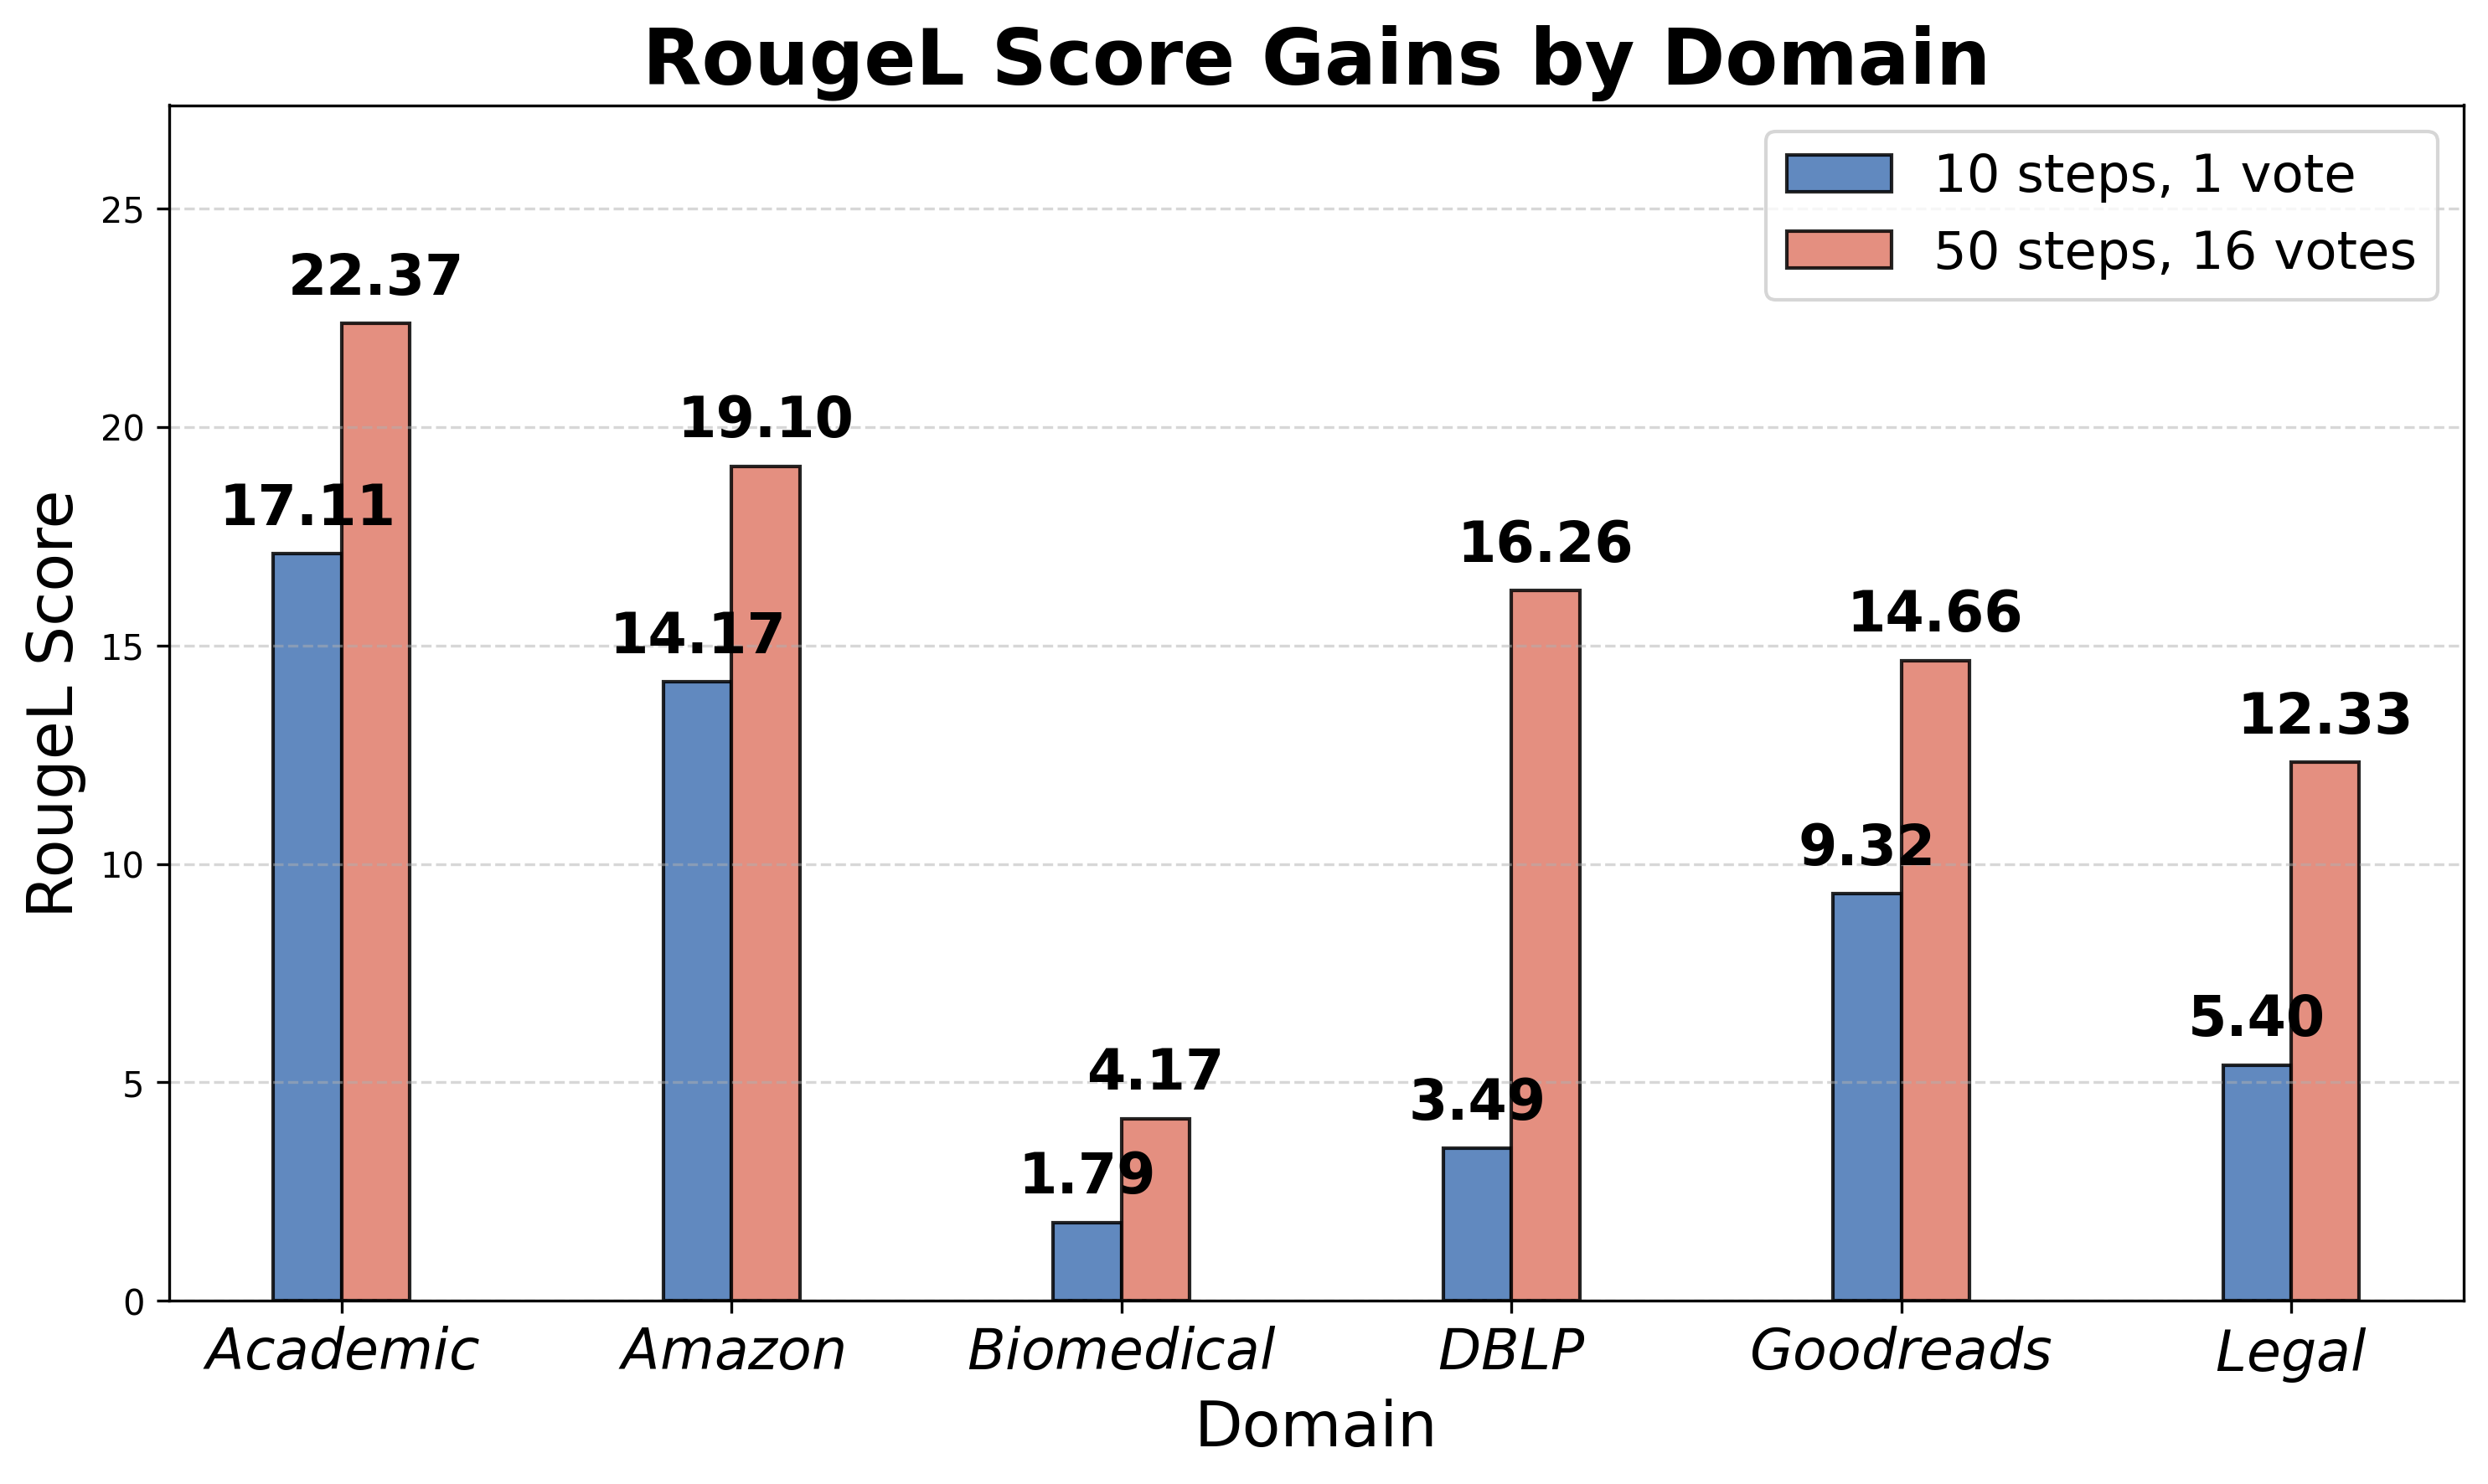
\includegraphics[width=\textwidth]{img/rougel_medium_hard_avg_domain_bar_chart.png}
%         \caption{RougeL scores on medium and hard questions}
%         \label{fig:multi-hoprougl}
%     \end{subfigure}
%     \caption{Performance improvements across domains with maximum inference scaling (50 steps, 16 votes) compared to no inference scaling (10 steps, 1 vote). Subfigure (a) reports F1 score gains on medium and hard questions, while (b) shows corresponding improvements in RougeL score. The results demonstrate consistent and substantial gains across all six domains, highlighting the effectiveness of inference scaling for complex question answering }
% \end{figure}

\begin{figure}[t]
\centering
    \includegraphics[width=\textwidth]{img/Inference_Scaled_GraphRAG_Edited.png}
    \caption{Overview of \textit{Inference Scaled GraphRAG}. The diagram illustrates the iterative process where a question is processed by an LLM. The LLM generates k thought-actions pairs. We perform majority voting to select the best action to interact with the knowledge graph. The response returned from the knowledge graph is fed back as context to the LLM for generation of the next thought-action pair. Generation continues until we reach an answer or hit the maximum step count}
    \label{fig:ISGR_overview}
\end{figure}

% \begin{figure}[t]
%     \centering
%     \begin{subfigure}[t]{0.48\textwidth}
%         \centering
%         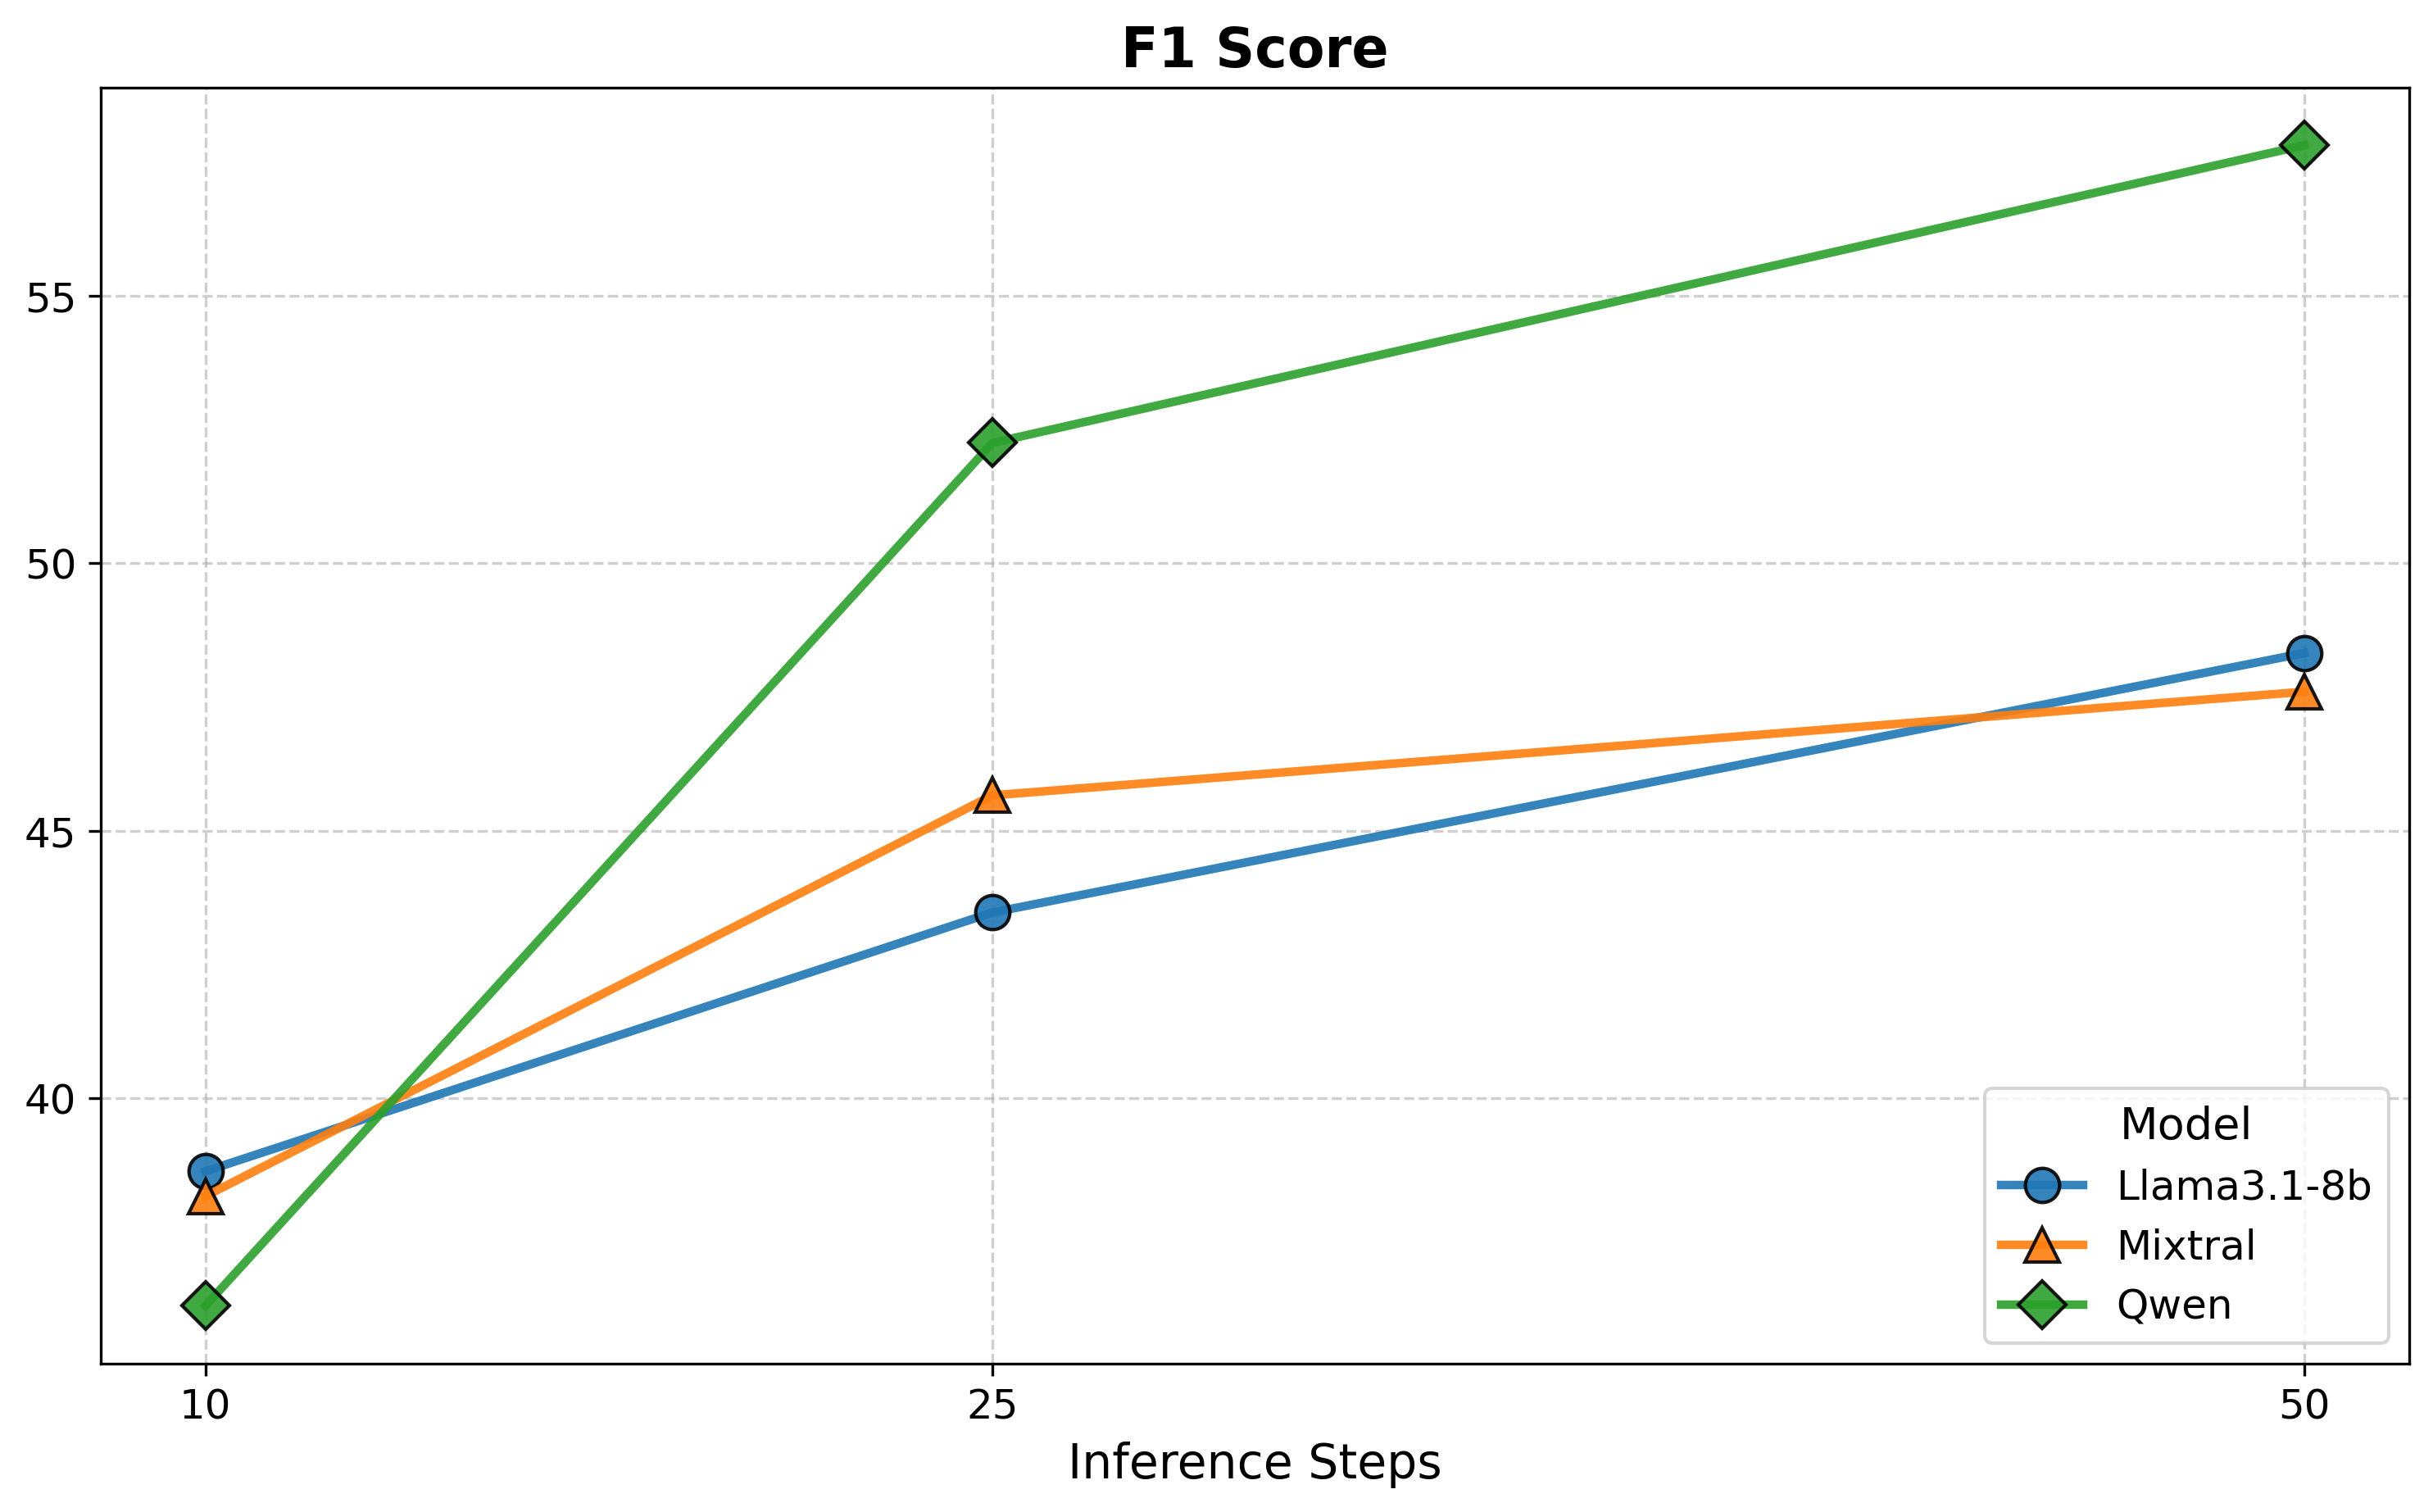
\includegraphics[width=\textwidth]{img/f1_score_majority_voting_1.png}
%         \caption{F1 Scores}
%         \label{fig:f1_scores}
%     \end{subfigure}
%     \hfill
%     \begin{subfigure}[t]{0.48\textwidth}
%         \centering
%         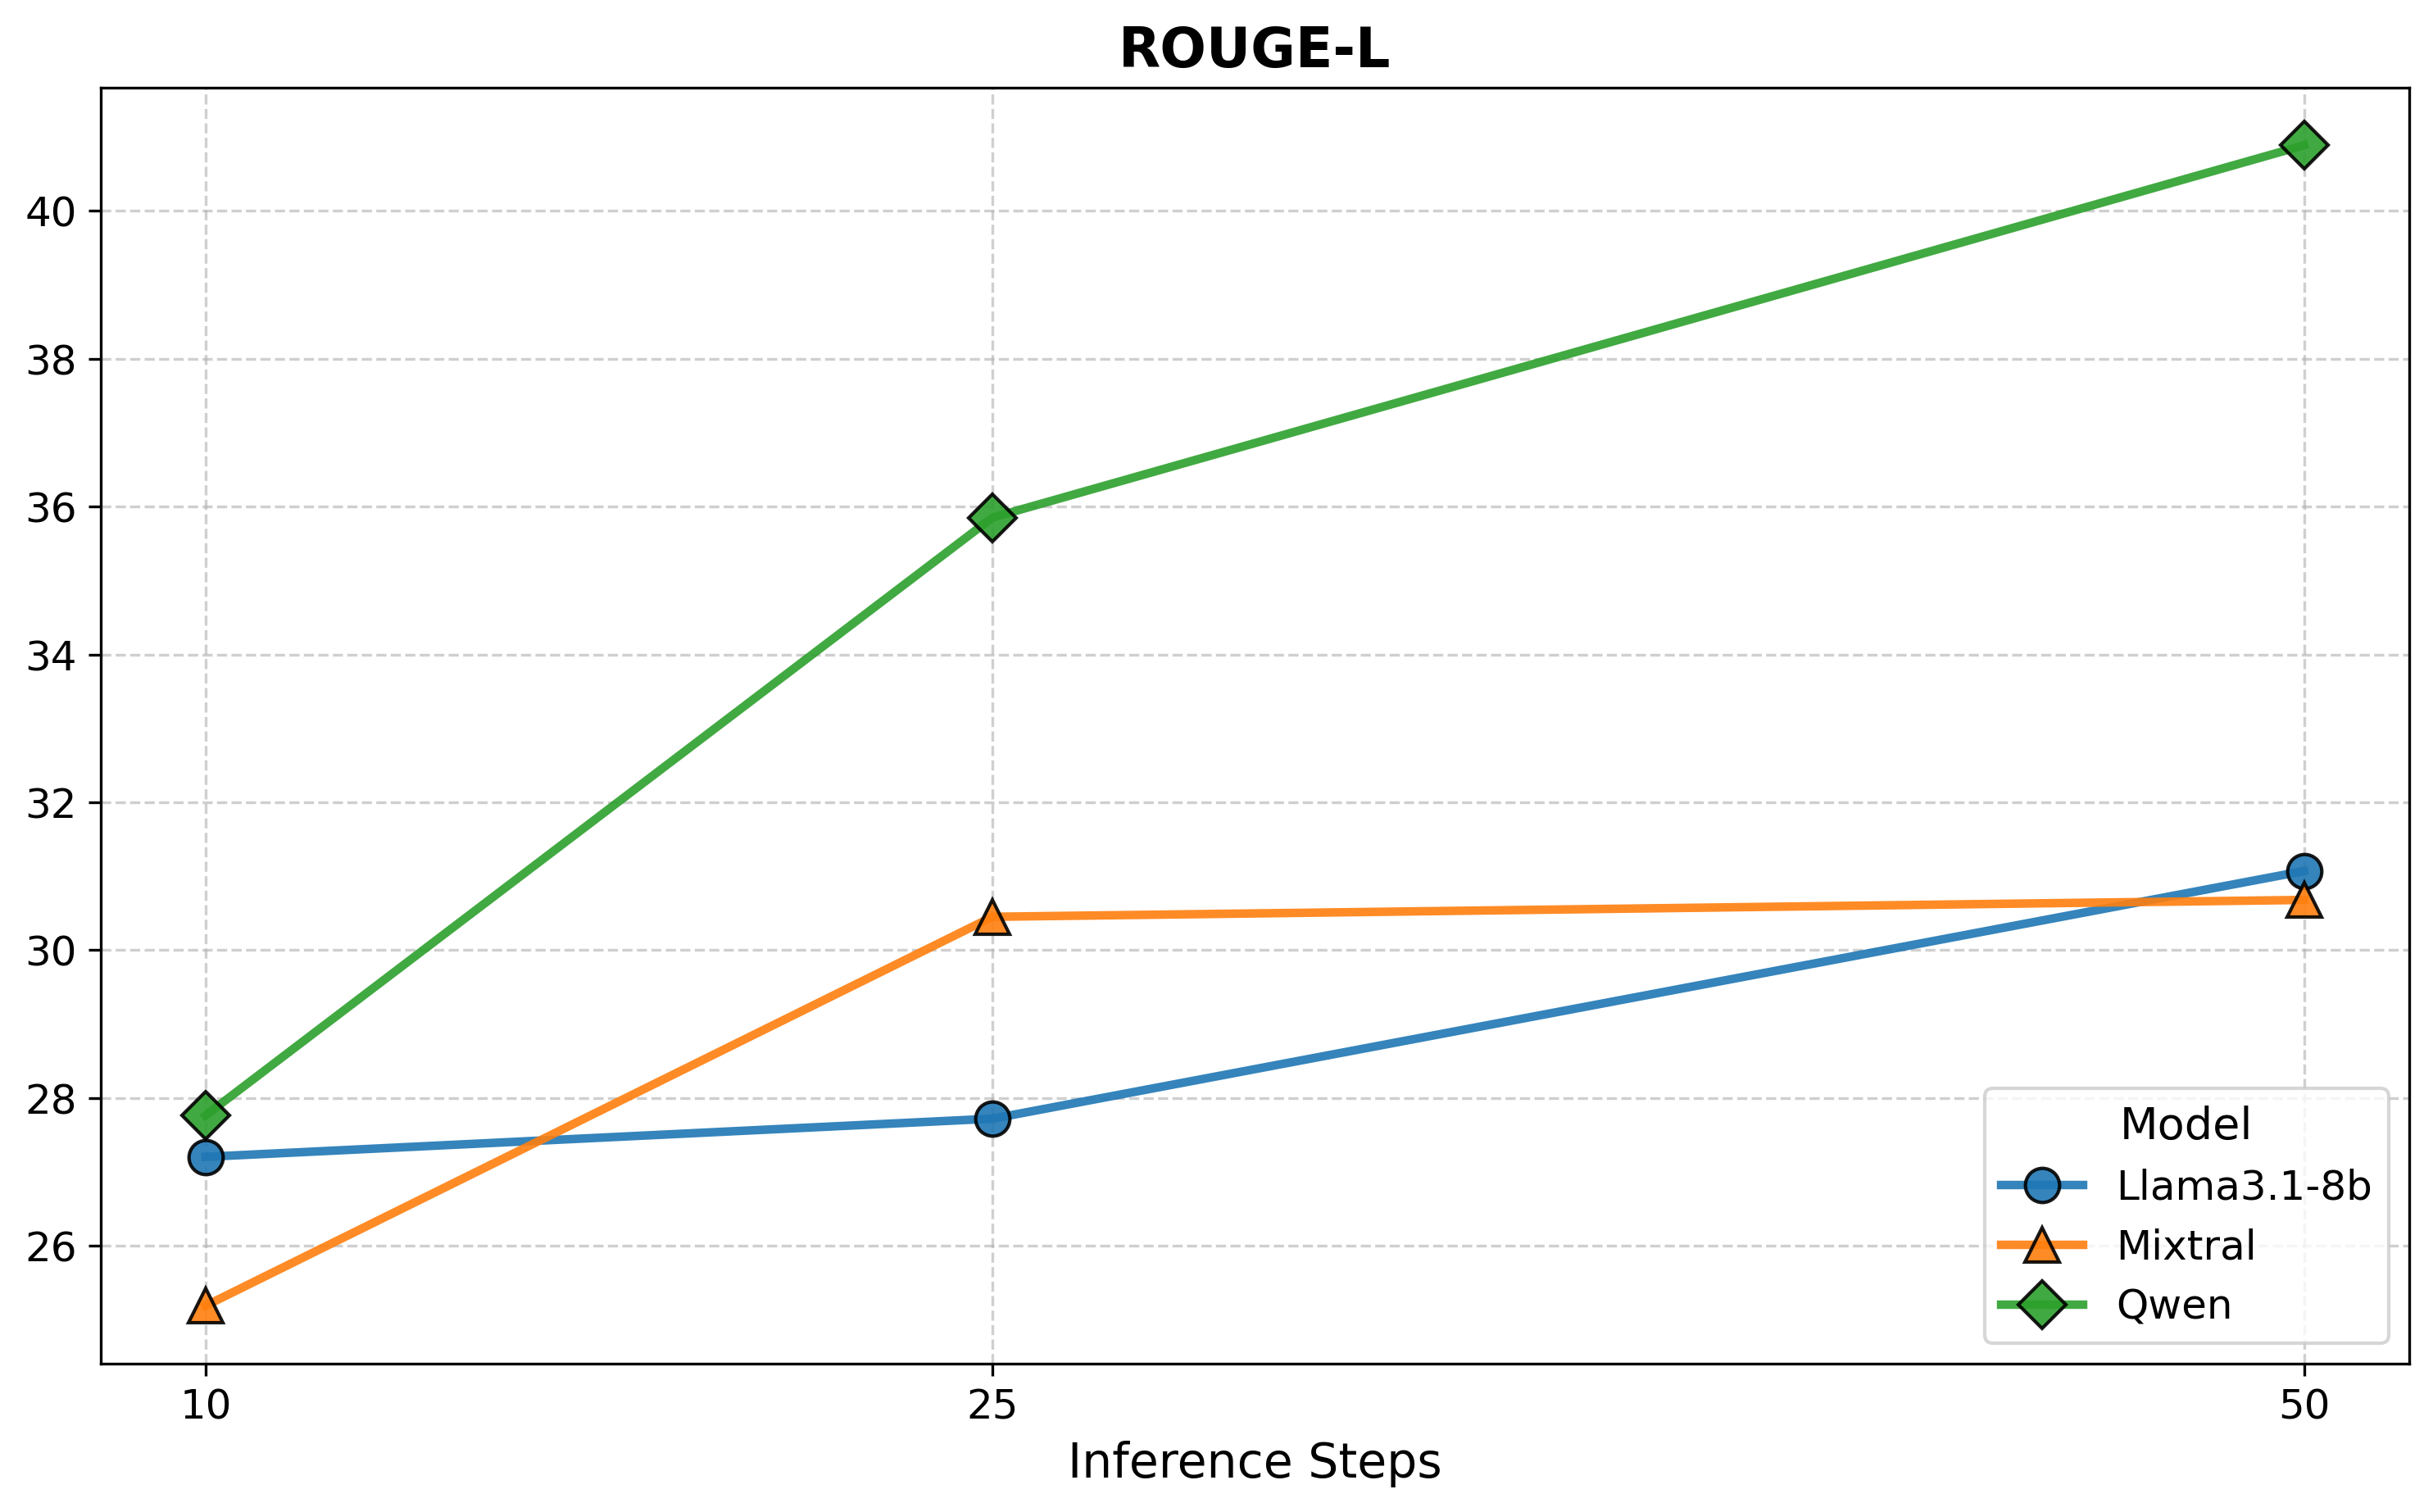
\includegraphics[width=\textwidth]{img/rougel_majority_voting_1.png}
%         \caption{ROUGE-L Scores}
%         \label{fig:rougeL_scores}
%     \end{subfigure}
%     \caption{Performance of \textit{Inference Scaled GraphRAG} under varying inference step counts and majority voting thresholds. 
%     \textbf{(a)} F1 score increases consistently with more inference steps across all voting configurations.  
%     \textbf{(b)} ROUGE-L scores show a similar trend, reflecting improvements in both symbolic and semantic alignment with ground-truth answers. 
%     Higher majority voting thresholds generally improve performance, highlighting the ability of both sequential scaling and parallel scaling to improve performance.}
%     \label{fig:combined_scores}
% \end{figure}

\paragraph{Reasoning.} Given a user query and the current context, the LLM first determines whether the question can be answered or whether additional information is required. If more information is needed, the model generates an intermediate goal. For example, for the question “Who are the authors of Language Models are Few-Shot Learners?”, the model may reason: “We need to first locate the node corresponding to the paper titled Language Models are Few-Shot Learners.”

\paragraph{Interaction.} Based on its reasoning, the LLM generates a function call to interact with the KG. We define a fixed set of functions the model can call \citep{yao2023reactsynergizingreasoningacting,jin2024graph}:
\begin{itemize}
\item RetrieveNode: Performs semantic search over the graph to retrieve the node most similar to a given query (equivalent to standard RAG).
\item NodeFeature: Returns the feature associated with a specified node.
\item NeighborCheck: Retrieves the neighbors of a given node along with edge information.
\item NodeDegree: Returns the degree of a node.
\end{itemize}
These functions define an interface between the LLM and the graph environment, effectively framing the LLM as a reasoning agent \citep{xi2023risepotentiallargelanguage, zhuang2023toolqa} operating over a structured space. This agent-like formulation allows us to explicitly control and scale the inference process, as described next.

\subsection{Inference-time scaling}

Multi-hop reasoning is essential in KG-based QA because critical information may be distributed across distant nodes. However, as the number of hops increases, the size of the relevant subgraph grows exponentially. LLMs often struggle with such compositional tasks due to limited context length and inference-time compute. QA performance degrades significantly on questions requiring multi-hop or inductive reasoning.

To address this, we introduce training free \citep{dong2024surveyincontextlearning} inference-time scaling strategies aimed at improving the reasoning ability of LLMs. These strategies are inspired by recent work showing that increasing inference-time compute can substantially improve LLM performance on tasks such as mathematical reasoning and program synthesis \citep{wu2025inference}. We consider two orthogonal axes of inference scaling:

\paragraph{Sequential scaling.} This approach increases the number of reasoning steps the model is allowed to take, thereby enabling deeper graph traversal. By extending the chain-of-thought, the model can accumulate intermediate knowledge, revise earlier assumptions, and explore the graph more effectively. In our setting, we increase the number of reasoning-interaction loops our model can perform before returning a response. This results in the model generating a much longer chain-of-thought and constructing more informed, contextually grounded answers by progressively integrating information across multiple hops in the knowledge graph.

\paragraph{Parallel scaling.} Parallel scaling enhances robustness by sampling multiple independent reasoning trajectories simultaneously and aggregating their outputs. We use majority voting over the sampled thought-action pairs \citep{brown2024largelanguagemonkeysscaling} to select the most consistent action. This approach improves reliability without the need for a learned verifier or extra supervision. In particular, we apply majority voting at the level of \texttt{Interaction} function calls, enabling us to identify and prioritize common reasoning paths across the sampled runs.

% \paragraph{Parallel scaling.} Parallel scaling improves robustness by sampling multiple independent reasoning trajectories in parallel and aggregating their outputs. We employ majority voting over the sampled thought-action pairs \citep{brown2024largelanguagemonkeysscaling} to select the best action. This strategy improves reliability without requiring a learned verifier or additional supervision. Specifically, we apply majority voting at the level of \texttt{Interaction} function calls, allowing us to identify and prioritize common reasoning paths across sampled runs.

\paragraph{Budget forcing.} Our formulation naturally supports budget forcing \citep{muennighoff2025s1simpletesttimescaling}, wherein we impose explicit limits on the number of reasoning steps (sequential scaling) and samples (parallel scaling) allowed during inference. This budget controls the computational cost and aligns with recent trends in controllable inference for LLMs. By tuning these parameters, we can trade off between performance and efficiency in a predictable manner.
